\section{The \texttt{omp barrier}}

Figure \ref{fig:fetchandadd} shows a simple barrier that can be used
for a OpenMP runtime system. Each arriving thread will decrease the
counter with an atomic operation, and they will spin checking the
counter value and not leave the barrier until the counter becomes zero.

\begin{figure*}[htbp]
  \begin{center}
    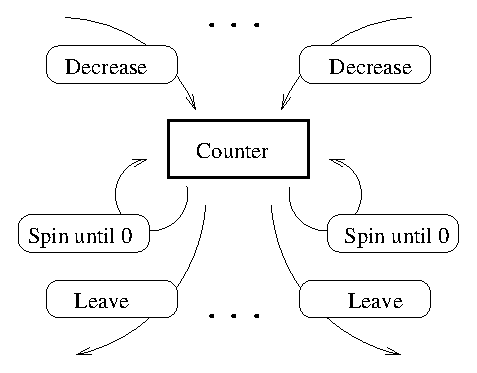
\includegraphics[angle=0, scale=.75]{fetchandadd.eps}
    \caption{Barrier implemented with fetch-and-add}
    \label{fig:fetchandadd}
  \end{center}
\end{figure*}

Algorithm \ref{alg:barrier} describes a more realistic implementation used 
in the XL OpenMP runtime system on AIX and Linux,

\begin{algorithm}[h]
  \SetLine
  \AlgData{Distributed counter with each element as one}
  \AlgData{Local sensor with each element as one}
  \BlankLine
  \Begin {
    Decrease my own distributed counter element\;
    \eIf{I am the master thread}{
      \Repeat{all distributed counter elements are zero} {
        \lForEach{element in distributed counter}{check if it is zero}
      }
      \ForEach{element in distributed counter}{set it back to one}
      \ForEach{element in local sensor}{set it to zero}
    }{
      \Repeat{it is zero} {
        check my local sensor element
      }
    }
    Set my own local sensor element back to one\;
  }
  \caption{Barrier with distributed counter and local sensor}
  \label{alg:barrier}
\end{algorithm}


Instead of having one counter, each thread will operate its own counter, thus
the expensive fetch and add operation can be replaced with a regular
add. In order to further reduce the contention, we also have a local
sensor to reduce the false sharing between reads from different
threads\cite{Zha03}.

\begin{figure*}[htbp]
  \begin{center}
    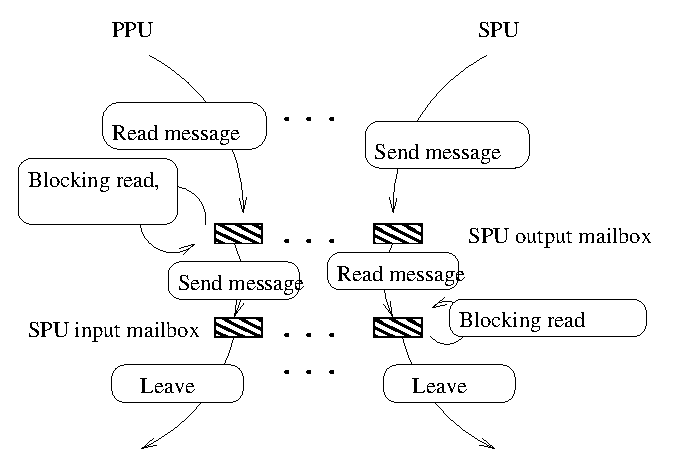
\includegraphics[angle=0, scale=.85]{combined.eps}
    \caption{Barrier with SPU output and input mailbox}
    \label{fig:combined}
  \end{center}
\end{figure*}

The algorithm can be mapped perfectly onto the Cell processor. The
distributed counter and local sensor can be replaced by the SPU output and
input mailbox separately. For example, the following code executed on an
SPU and achieve the algorithm drawn in Figure \ref{fig:combined}.

{\small
\begin{verbatim}
  {
    int data;
    spu_writech(SPU_WrOutMbox, 1);
    data = spu_readch(SPU_RdInMbox);
  }
\end{verbatim}
}

And the PPU version,

{\small
\begin{verbatim}
  unsigned int data;
  spe_context_ptr_t id = _xlbesplitSPUThreads[i].spuid;

  for (int i=0; i<num_threads; i++) {
    while(spe_out_mbox_status(id) == 0);
    spe_out_mbox_read(id, &data, 1);
  }

  for (int i=0; i<num_threads; i++) {
    while (spe_in_mbox_status(id) == 0);
    spe_in_mbox_write(id, &data, 1, SPE_MBOX_ANY_NONBLOCKING);
  }
\end{verbatim}
}

In the real implementation, a barrier is also a chance for PPU and SPU to 
exchange data such as for handling single, reduction, copyprivate etc. 

%We used the EPCC microbenchmarks\cite{Bul99} to show the performance
%gains coming from optimization considerations discussed above.
%
%The EPCC benchmarks have two parts: the synchronization suite and the
%schedule suite. Since we are concentrating on workshare
%implementation, we have focused on the synchronization benchmark. It
%includes separate test cases for parallel region, workshares 
%
%\emph{Testing results to be added \ldots}

%For a parallel region, as we show in Figure \ref{fig:compare}, the ``on
%demand'' initialization method introduced in section
%\ref{sec:optimize} reduces its overhead on both POWER3 and POWER4
%systems. 
